
\chapter {Getting Started}
\label{chap4}

In this chapter we will get started with Oscad. We will run through the various options available with an example circuit. Refering to this chapter will make you familiarize with Oscad thereby helping you plan your project before actually designing a circuit. Lets get started.

%\section{Oscad main window}
After you finish installing Oscad, a shortcut link for Oscad will be created on your desktop. You will click on this link to launch oscad. Oscad main window will open up. It is shown in Figure \ref{main-window}. On the menu bar there are two options, {\tt Project} and {\tt Help}. To create a new project or open an existing project, use the project option.

\begin{figure}
\begin{center}
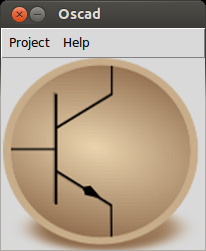
\includegraphics[width=0.5\linewidth]{figures/main-window.png}
\caption{Oscad main window}
\label{main-window}
\end{center}
\end{figure}

Let us open an existing project. Click on Project and select Open. The {\tt Choose Directory} window opens up. This window is shown in figure \ref{open-directory}. Choose the corresponding directory of the project. Choose {\tt RC} example from the Examples folder that you have downloaded from the Oscad webpage. Click on OK. Another window will open asking to enter the Project Name. This window is illustrated in figure \ref{project-name}. Since we are opening an already existing project, the name will appear in the text box automatically. In case you are creating a new project then you have to write the name of your new project in this window. Click on OK after you finish doing it.

\begin{figure}
\begin{center}
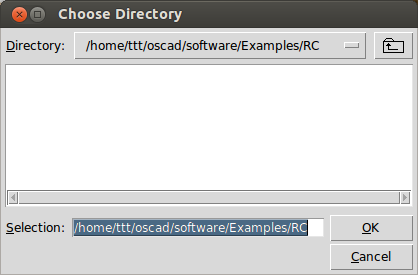
\includegraphics[width=0.5\linewidth]{figures/open-project-directory.png}
\caption{Open project directory}
\label{open-directory}
\end{center}
\end{figure}

\begin{figure}
\begin{center}
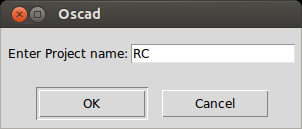
\includegraphics[width=0.5\linewidth]{figures/project-name.png}
\caption{'Enter Project Name' window}
\label{project-name}
\end{center}
\end{figure}



\begin{figure}
\begin{center}
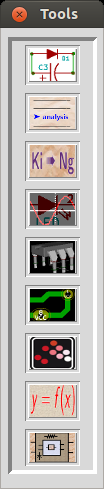
\includegraphics[width=0.2\linewidth]{figures/tool-window.png}
\caption{Oscad Tool bar}
\label{tool-window}
\end{center}
\end{figure}

%\section{Oscad Tool Bar}
After you finish creating a new project or opening a new project, a vertical tool bar\index{Oscad tool bar} will appear. This tool bar is shown in figure \ref{tool-window}. This is the {\tt Oscad tool bar}. It contains 9 tools. These tools have images depicting their purpose. If you place your mouse pointer on these tools, the name of the tool appears at the bottom of the mouse pointer. Following is the list of tools,  from top to bottom as they appear, in the Oscad tool bar.

\begin{enumerate}
\item Schematic Editor
\item Analysis Inserter
\item Netlist Converter
\item Ngspice
\item Footprint editor
\item Layout Editor
\item SMCSim
\item Model builder
\item Subcircuit builder
\end{enumerate}

\section{Schematic Editor}
Click on the first tool on the tool bar i.e. Schematic Editor\index{Schematic!editor}. Doing so will open EESchema, the schematic editor used in Oscad. If you had started a new project, you will get the schematic editor window with an info dialog box. This is illustrated in figure \ref{schematic-editor-newprj}. This warning can be safely ignored by clicking on {\tt OK}. 

However, if you had opened an already existing project, you will get the schematic editor window along with a Load error\index{Load error message}. This is illustrated in figure \ref {schematic-editor-existing}. This error occurs because the schematic that you have opened has not been loaded with the libraries mentioned in the Load Error message. Close the Load Error message by clicking on the {\tt close} button. The RC circuit diagram opens up as shown in figure \ref{eeschema}. You are now ready to start creating/editing the circuit schematic. To know how to use the schematic editor to create circuit schematics, refer to Chapter \ref{chap5}.

\begin{figure}
\begin{center}
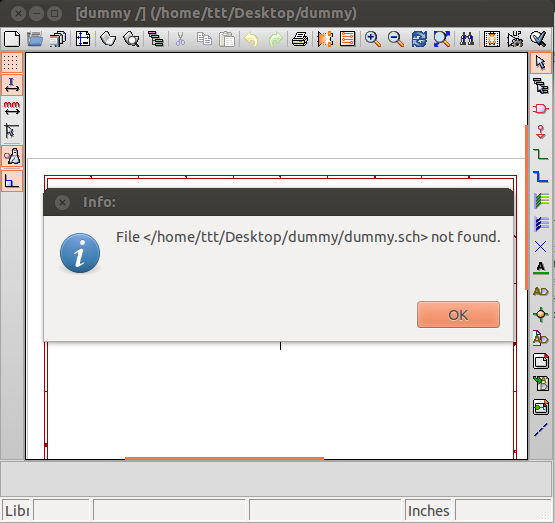
\includegraphics[width=0.8\linewidth]{figures/schematic-editor-newprj.png}
\caption{Schematic Editor (opening a new project)}
\label{schematic-editor-newprj}
\end{center}
\end{figure}


\begin{figure}
\begin{center}
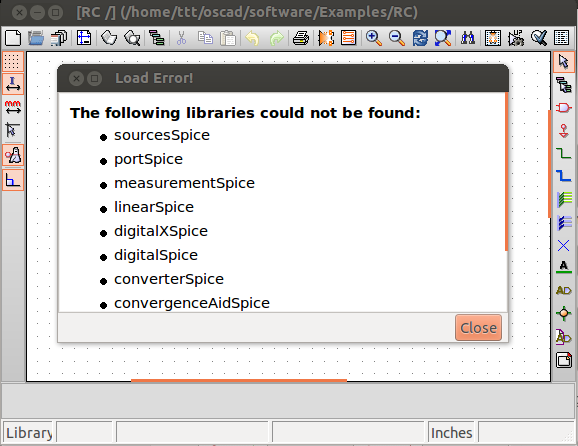
\includegraphics[width=0.8\linewidth]{figures/schematic-editor-existingprj.png}
\caption{Schematic Editor (opening an already existing project)}
\label{schematic-editor-existing}
\end{center}
\end{figure}



\begin{figure}
\begin{center}
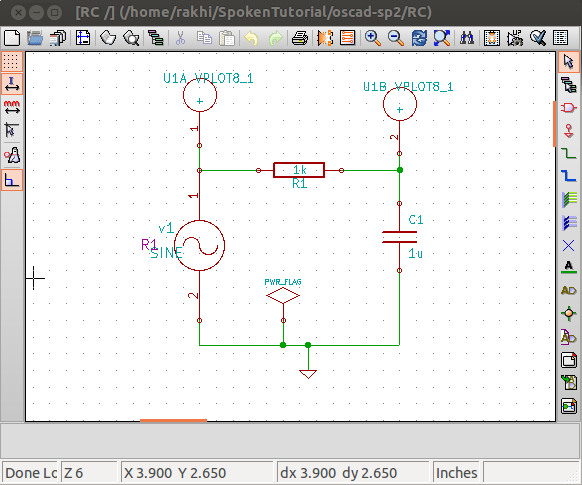
\includegraphics[width=0.8\linewidth]{figures/eeschema.png}
\caption{Schematic Editor (with RC circuit)}
\label{eeschema}
\end{center}
\end{figure}



\section{Analysis Inserter}\label{subsec-analyis-inserter}

The second tool on the tool bar is the Analysis Inserter\index{Analysis Inserter}. It is necessary that before you use this tool, you have the spice netlist file (.cir) created. This is because this tool is used to insert analysis commands to the spice netlist file. To know how to generate the spice netlist file, refer to the section \ref{chap5-netlist-generation}.

When you click on this tool, a window named {\tt kicad Ngspice} will open. This is the Analysis inserter GUI. It is shown in figure \ref{analyis-inserter}. This window will allow the analysis commands to be inserted in to the spice netlist file. The use of analysis inserter is explained in detail in section \ref{ana}.

\begin{figure}
\begin{center}
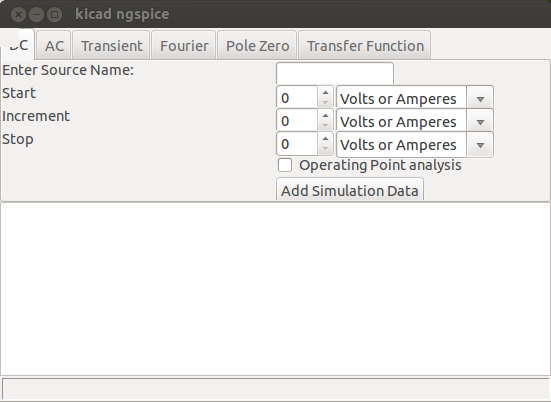
\includegraphics[width=0.8\linewidth]{figures/analysis-inserter.png}
\caption{Analyis Inserter}
\label{analyis-inserter}
\end{center}
\end{figure}

\section{Netlist Converter}\label{subsec-netlist-converter}

The third tool on the tool bar is the {\tt Netlist Converter}\index{Netlist converter}. Before you use this tool, you should have already created the spice netlist file and used analysis inserter to generate analysis commands. To know how to generate spice netlist, refer to the section \ref{chap5-netlist-generation}. This file is not directly usable for simulation. In other words, it is not compatible with Ngspice.

 The spice netlist file contains only the component placement information and it says nothing about the magnitude and other parameters (if applicable) of the source components like voltage source, current source etc. When you click on the {\tt Netlist Converter} tool, a terminal window will open up as shown in figure \ref{netlist-converter}. If you observe this terminal window, you will notice that it first tells you which .cir file it is referring to. It also asks for the source value. It may ask other parameters too depending upon the type of sources used. Once you are done entering the values, press the `Enter' key. It will generate {\tt .cir.out} and {\tt .cir.ckt} files in the same project directory.


\begin{figure}
\begin{center}
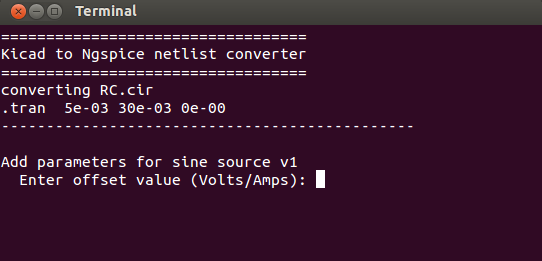
\includegraphics[width=0.8\linewidth]{figures/netlist-converter.png}
\caption{Netlist Converter}
\label{netlist-converter}
\end{center}
\end{figure}

\section{Ngspice}
The sections \ref{subsec-analyis-inserter} and \ref{subsec-netlist-converter} helped to generate a netlist suitable to be simulated using Ngspice\index{Ngspice}. Clicking on the tool {\tt Ngspice} will open a terminal window and a plot window as shown in figure \ref{Ngspice-simulation}. You should have the converted netlist file `.cir.out' before using this tool.


\begin{figure}
\begin{center}
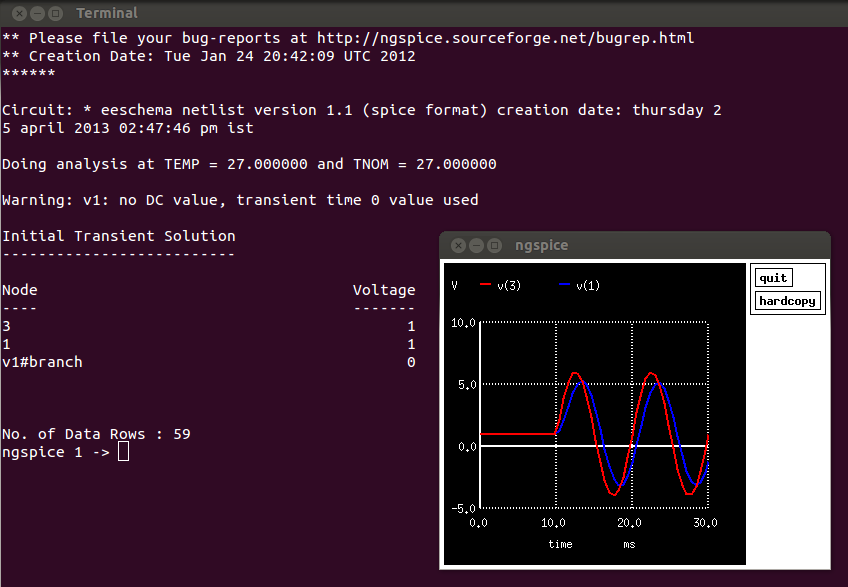
\includegraphics[width=0.8\linewidth]{figures/ngspice-simulation.png}
\caption{Ngspice Simulation}
\label{Ngspice-simulation}
\end{center}
\end{figure}

\begin{figure}
\begin{center}
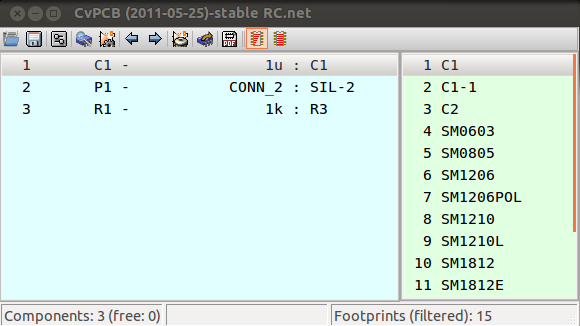
\includegraphics[width=0.8\linewidth]{figures/CvPCB-window.png}
\caption{CvPcb window}
\label{CvPcb-window}
\end{center}
\end{figure}

\section{Footprint Editor}
Clicking on the {\tt Footprint Editor} tool will open the {\tt CvPcb} window. This window will ideally open the .net file for the current project. So for using this tool, you should have the netlist for PCB design (a .net file). To know more about how to create netlist for PCB, refer to the section \ref{netc}.

On clicking the Footprint editor tool, we see the corresponding .net file for RC circuit. This window is shown in figure \ref{CvPcb-window}. 

The main purpose of this window is to let you choose the footprints for the various components of your circuit. Let us view the footprint {\tt C1} for capcitor C1. Click on C1 from the right hand side of CvPcb window. Click on {\tt View Selected Footprint} tool from the tool bar of CvPcb\index{CvPcb} window,. This will show the footprint corresponding to C1. This is illustrated in Figure \ref{footprint-c1}. To know more about how to assign a footprints\index{Footprints} to components, see Chapter \ref{chap7}.

\begin{figure}
\begin{center}
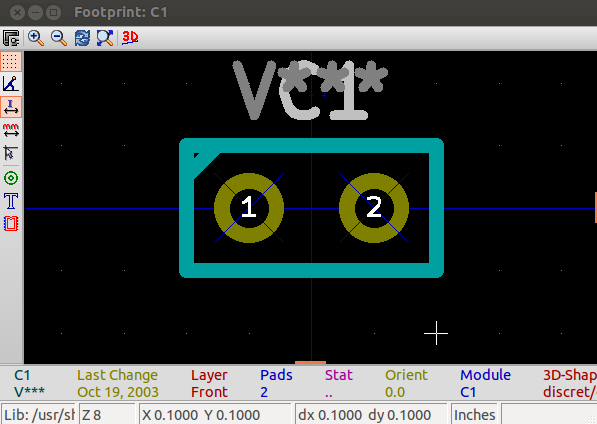
\includegraphics[width=0.8\linewidth]{figures/footprint-c1.png}
\caption{Footprint for C1}
\label{footprint-c1}
\end{center}
\end{figure}

\section{Layout Editor}
Clicking on the {\tt Layout Editor} tool will open {\tt Pcbnew}\index{Pcbnew}, the layout editor used in Ocad. In this window, you will create the PCB. It involves laying tracks and vias, performing optimum routing of tracks, creating more than one copper layer for PCB etc. An already made PCB design for RC circuit is shown in figure \ref{pcb-RC}. This is how the PCB will look like when you actually print it on a copper-clad board. When you save this design, it will be saved as a .brd file in the same directory. Chapter \ref{chap7} explains how to use the Layout Editor to design a PCB.

\begin{figure}
\begin{center}
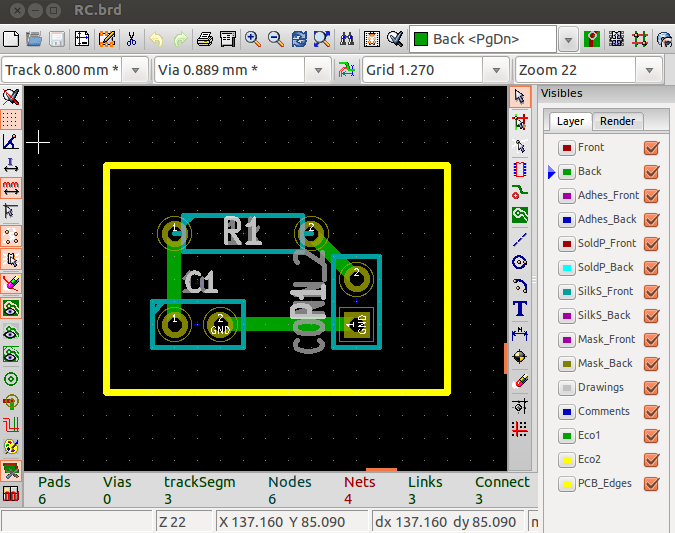
\includegraphics[width=0.8\linewidth]{figures/pcb-rc.png}
\caption{PCB design for RC circuit}
\label{pcb-RC}
\end{center}
\end{figure}


\section{SMCSim}

SMCSim stands for Scilab Based Mini Circuit Simulator. This tool will generate mathematical equations for your circuit, thereby helping you gain a better understanding of your circuit. Oscad uses Scilab for this purpose \cite{scilab}. Clicking on this tool will open a small window where you will have to choose between three options.
\begin{enumerate}
\item Normal
\item Symbolic
\item Matrix
\end{enumerate}
These are basically the modes used for circuit simulation. This window is illustrated in figure \ref{scilab-mode}. After you select one of them and click ok, Scilab will be launched automatically. Let us choose {\tt Symbolic}.  The scilab console will show the set of equations for the circuit as shown in Figure \ref{scilab-window}. A plot window will also open showing the plot of variables of the circuit. Which variables to plot depends upon the placement of plot components in the circuit schematic. The plot window is shown in figure \ref{scilab-plot}. To know more about how to use this feature, refer Chapter \ref{chap9}.

\begin{figure}
\begin{center}
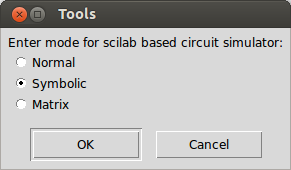
\includegraphics[width=0.5\linewidth]{figures/scilab-mode.png}
\caption{Window to choose the mode for Scilab based circuit simulator}
\label{scilab-mode}
\end{center}
\end{figure}

\begin{figure}
\begin{center}
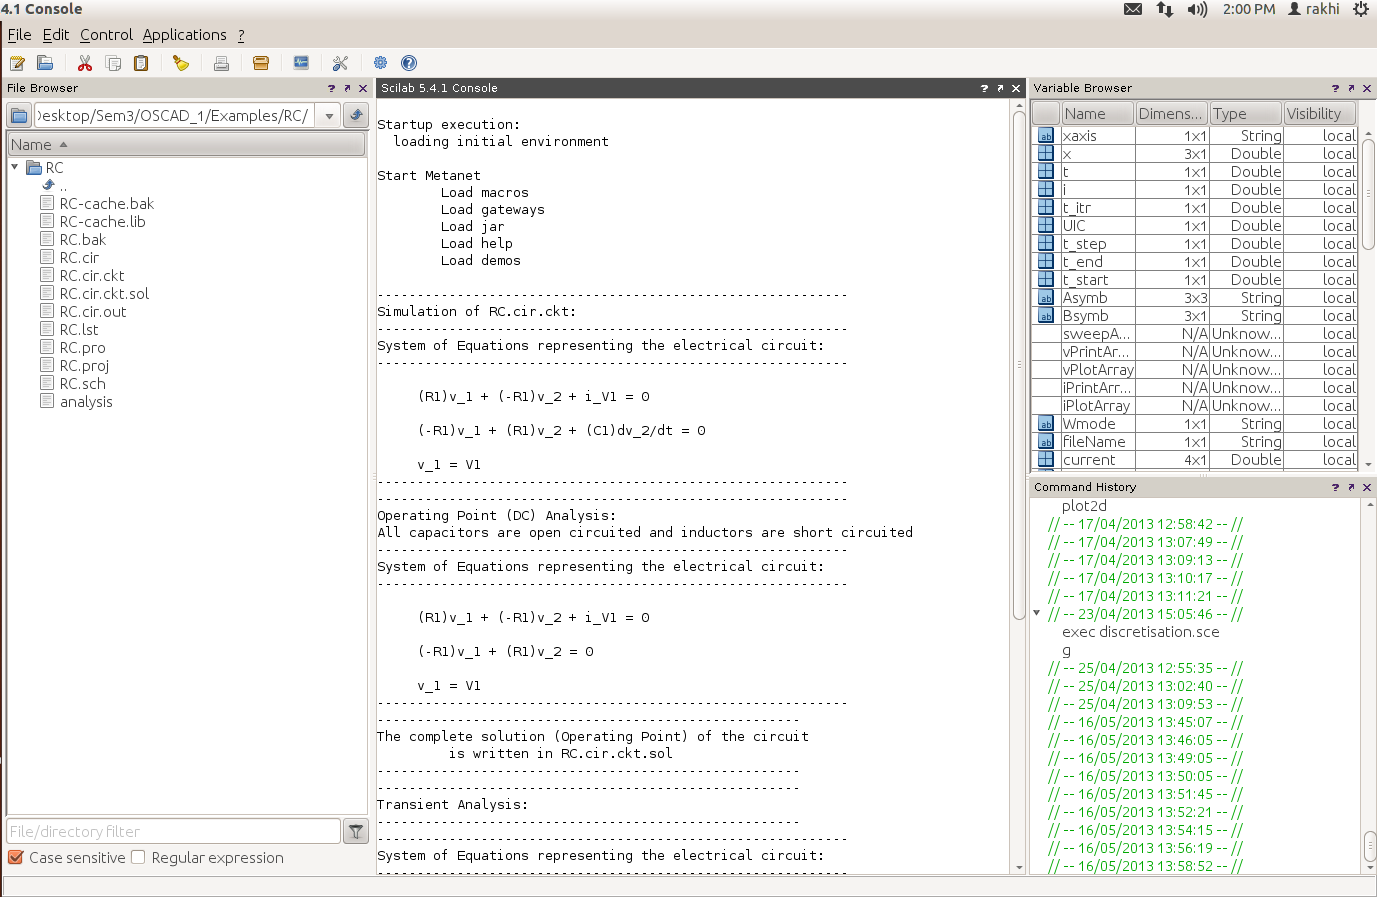
\includegraphics[width=\linewidth]{figures/scilabRC.png}
\caption{Scilab Window showing system of equations representing the electrical circuit}
\label{scilab-window}
\end{center}
\end{figure}

\begin{figure}
\begin{center}
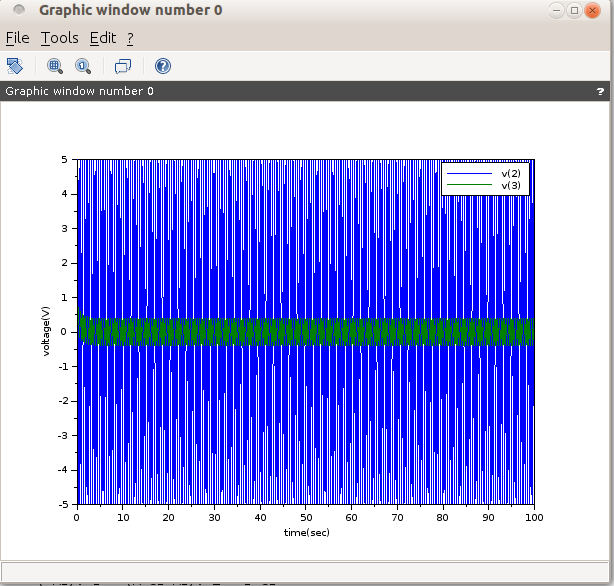
\includegraphics[width=0.5\linewidth]{figures/scilabFig.png}
\caption{Plot window of Scilab showing the result of the circuit simulation}
\label{scilab-plot}
\end{center}
\end{figure}


\section{Model builder}

Oscad also gives you an option to re-configure the model of a component. It facilitates the user to change the model of components such as diode, transistor, MOSFET etc. When you click on the {\tt Model builder} tool, you will get the window as shown in figure \ref{model-builder-blank}. You see a blank window because the RC  circuit which you have opened does not have any component whose model can be edited. If suppose you had a diode (say {\tt 1N4007}) in the circuit then the model builder window would have looked like as shown in figure \ref{model-builder-diode}. We can see that it shows {\tt 1n4007} in the window. After choosing {\tt 1n4007} and clicking on OK, it will confirm saying {\tt Do you want to edit?}. After clicking on OK, a window will open. This window will contain the various parameters governing the model of diode, for example reverse breakdown voltage (BV), ohmic resistance (RS) etc. This is illustrated in figure \ref{diode-model}. To know more about how to use this feature, refer chapter \ref{chap8}.

\begin{figure}
\begin{center}
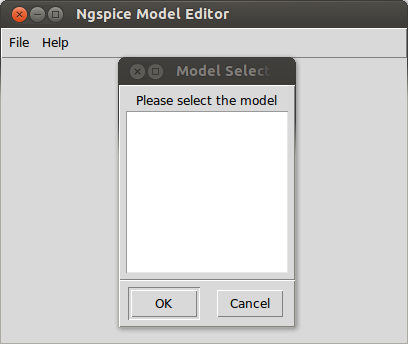
\includegraphics[width=0.5\linewidth]{figures/model-builder.png}
\caption{Model builder window}
\label{model-builder-blank}
\end{center}
\end{figure}

\begin{figure}
\begin{center}
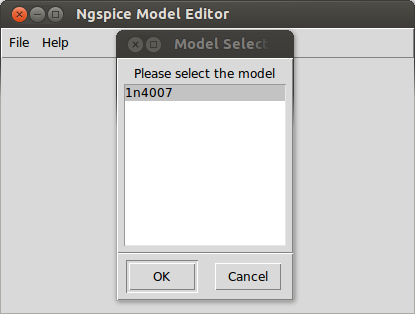
\includegraphics[width=0.5\linewidth]{figures/model-builder-diode.png}
\caption{Model builder window of circuit having a diode}
\label{model-builder-diode}
\end{center}
\end{figure}

\begin{figure}
\begin{center}
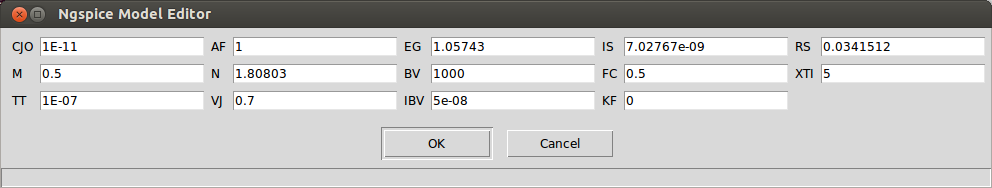
\includegraphics[width=\linewidth]{figures/diode-model.png}
\caption{Model builder window showing model of diode}
\label{diode-model}
\end{center}
\end{figure}

\section{Subcircuit builder}

Oscad gives you an option to build subcircuits. The subcircuits can again have components having subcircuits and so on. This enables users to build commonly used circuits as subcircuits and then use it across circuits. For example, one can build a 12 Volt power supply as a subcircuit and then use it as just a single component, across circuits without having the need to recreate it. Clicking on {\tt Subcircuit builder} tool will allow you to edit or create a subcircuit. To know how to make a subcircuit, refer to Chapter \ref{chap8}. Figure \ref{lm555n-subcircuit} shows the subcircuit of 555 timer IC.

\begin{figure}
\begin{center}
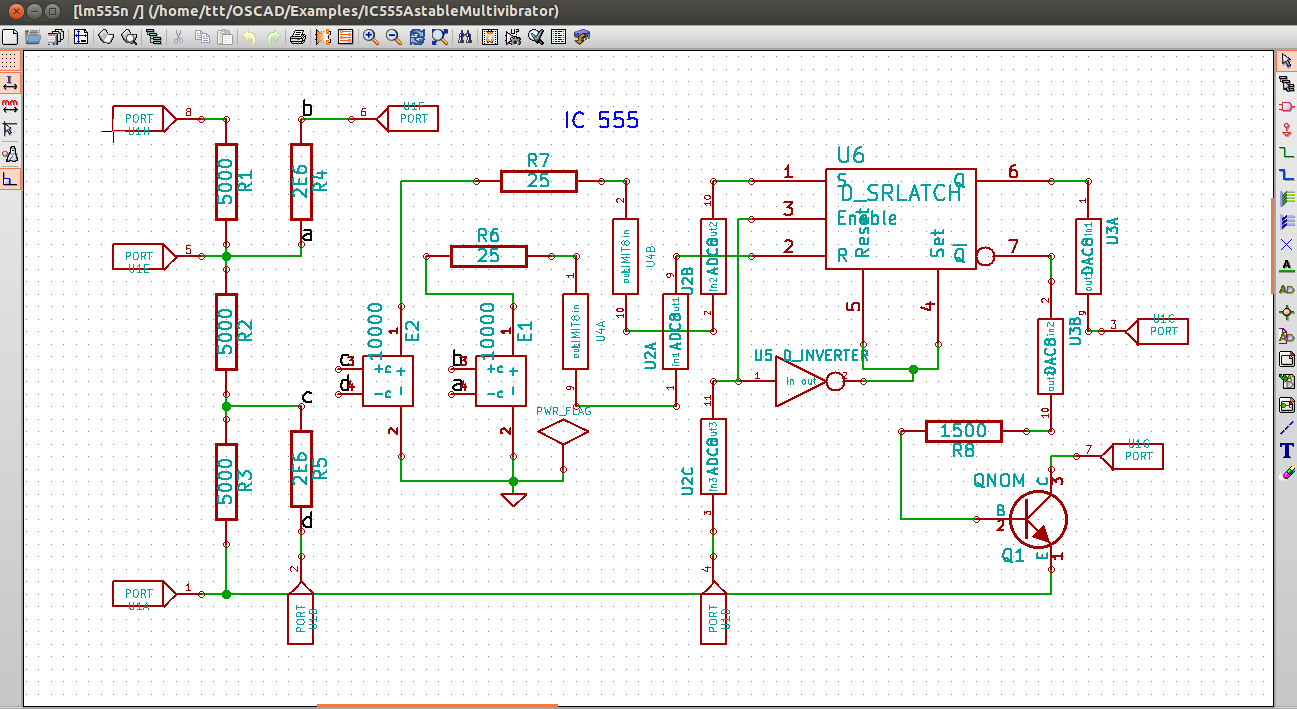
\includegraphics[width=\linewidth]{figures/subcircuit.png}
\caption{Subcircuit of 555 timer IC}
\label{lm555n-subcircuit}
\end{center}
\end{figure}
